\apendice{Estudio experimental}
Durante la realización del proyecto, no se ha realizado un estudio experimental. 

La realización de este seria esencial en un futuro cuando se haya obtenido un dispositivo final antes de lanzarlo al mercado. 

Sería útil realizar un estudio con un conjunto de pacientes para hacer un seguimiento de los datos recogidos por el dispositivo y observar cómo evolucionan desde la primera sesión hasta que finalmente se les da de alta.
De esta manera, se podría observar si las sesiones están resultado positivas o, en caso contrario, determinar si deberían interrumpirse para que un nuevo paciente en lista de espera pueda acceder a las sesiones de terapia.

\section{Configuración y parametrización de las técnicas.}

Para una correcta cuantificación de la fuerza ejercida a los sensores se ha realizado una parametrización de los sensores de fuerza resistivos. 

Al emplear este tipo de sensores para medir, la relación entre el nivel de cuantificación y la magnitud del peso no se comporta de manera lineal, sino que la curva característica muestra un comportamiento exponencial o logarítmico. 

En este proceso, primero se ha hecho una relación entre 10 pesos y el valor leído por el sensor (véase tabla \ref{tab:Relación Valor-Peso}). 
\begin{table}[h]
    \centering
    \begin{tabular}{|c|c|}
    \rowcolor[HTML]{BFBFBF} 
        \hline
        \textbf{Valor} & \textbf{Peso (kg)} \\ \hline
        0   & 0    \\ \hline
        165 & 0.5  \\ \hline
        258 & 1    \\ \hline
        302 & 1.5  \\ \hline
        340 & 2    \\ \hline
        368 & 2.5  \\ \hline
        404 & 3    \\ \hline
        440 & 3.5  \\ \hline
        460 & 4    \\ \hline
        498 & 4.5  \\ \hline
   \end{tabular}
    \caption{Relación Valor-Peso}
    \label{tab:Relación Valor-Peso}
\end{table}
Dado que solo se han obtenido diez valores experimentales, los valores que se encuentren entre dos de estos se determinan mediante interpolación lineal, que sigue la siguiente fórmula:
\begin{equation}
    y = \frac{y_1 - y_0}{x_1 - x_0} \cdot (x - x_0) - y_0
    \label{eq: Interpolación lineal}
\end{equation}

Dado que utilizamos este tipo de ecuación, los resultados no son 100\% reales, pero sí aproximados.

En la figura \ref{fig:Grafica peso-valor} se puede observar cómo crece la curva que relaciona los valores medidos con los pesos. El crecimiento de los primeros valores es considerablemente más pronunciado en comparación con los valores obtenidos con pesos más altos, lo cual se debe al comportamiento característico de los sensores de fuerza resistivos. 
\begin{figure}
    \centering
    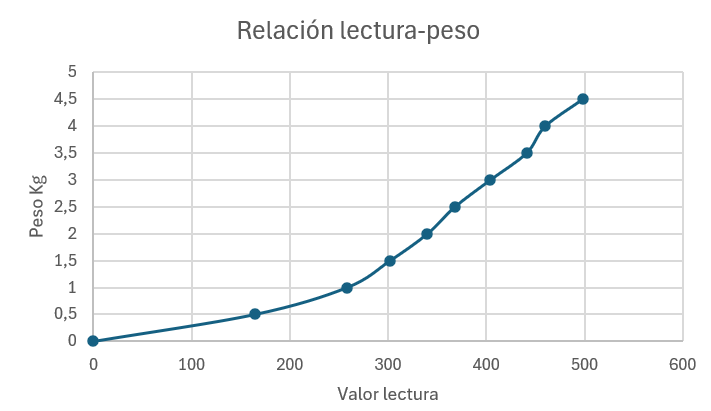
\includegraphics[width=0.75\linewidth]{img/Grafica peso-valor.png}
    \caption{Gráfica peso-valor. Fuente propia}
    \label{fig:Grafica peso-valor}
\end{figure}

Dado que al medir la fuerza ejercida se pueden crear picos máximos o mínimos falsos, se ha implementado la fórmula de la desviación estándar.
\begin{equation}
    \sigma=\sqrt{\frac{\sum\left(x_{i}-\mu\right)^{2}}{N}}
\end{equation}
Donde sigma es la desviación estándar, mu es la media, xi es cada valor muestreado y N es el total muestreado.